\section{Partie pratique}

\subsection{Contexte}
Dans un magasin où un système de caisses automatiques est mis en place, et suite à des cas de plus en plus fréquents de vol, les gérants du magasins décident de mettre en place un système de contrôle automatisé des marchandises lorsque les clients posent sur le comptoir basé sur le poids. Malheureusement, le système purement mécanique -- designé par des micro-techniciens -- n'arrive pas à différentier les bouteilles de boissons gazeuses de même volume. On vous demande alors -- à vous qui savez réfléchir -- de créer un programme simple qui permette de distinguer précisément et rapidement entre les bouteilles suivantes :

\vspace{0.2cm}
\noindent
\begin{minipage}[c]{\textwidth}
  \centering
  \makebox[\textwidth]{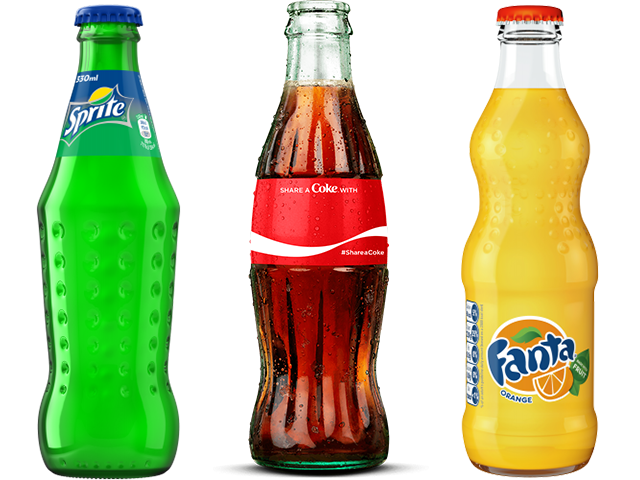
\includegraphics[width=\linewidth]{addOns/bouteilles.png}}\\
  \captionof{figure}{Bouteilles à détecter}
  \label{fig.Bouteilles}
\end{minipage}\\

\vspace{0.2cm}
Utilisez vos compétences d'experts en vision industrielle pour créer une programme tournant sur 3 modes distincts qui permette de détecter alternativement :

\vspace{0.2cm}
\begin{itemize}
  \item la position d'une bouteille de Sprite
  \item la position d'une bouteille de Fanta
  \item la position d'une bouteille de Coca
\end{itemize}


\newpage
\subsection{Résultats attendus}
Que le programme affiche un texte "MarqueDeLaBoissonGazeuse" (soit "Sprite", "Fanta" ou "Coca" correspondant au mode choisi) à l'emplacement où la bouteille se trouve.

\vspace{0.2cm}
\noindent
\begin{minipage}[c]{\textwidth}
  \centering
  \makebox[\textwidth]{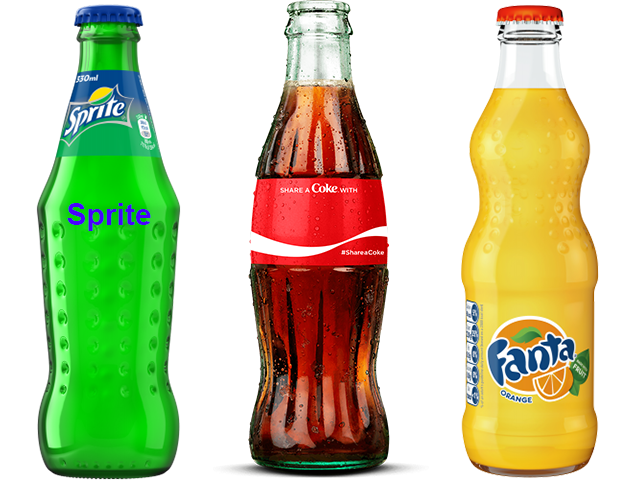
\includegraphics[width=\linewidth]{addOns/resultats.png}}\\
  \captionof{figure}{Résultats en mode "Sprite"}
  \label{fig.Bouteilles_Resultats}
\end{minipage}\\
